%%%%%%%%%%%%%%%%%%%%%%%%%%%%%%%%%%%%%%%%%%%%%%%%%%%%%%%%%%%%%%%%%%%%%%%%%%%%%%%%
%2345678901234567890123456789012345678901234567890123456789012345678901234567890
%        1         2         3         4         5         6         7         8

\documentclass[letterpaper, 10 pt, conference]{ieeeconf} 

\IEEEoverridecommandlockouts                              % This command is only
                                                          % needed if you want to
                                                          % use the \thanks command
\overrideIEEEmargins
% See the \addtolength command later in the file to balance the column lengths
% on the last page of the document

\usepackage{bm}
\usepackage{url}
\usepackage{tikz}
\usepackage{cite}
%\usepackage{dsfont}
\usepackage{textcomp}
\usepackage{upgreek}
\usepackage{footnote}
\usepackage{verbatim}
\usepackage{mathrsfs} 
\usepackage{graphicx}
\usepackage{paralist}
\usepackage{algorithm}
%\usepackage{algorithmicx}
\usepackage{algpseudocode}
\usepackage{tcolorbox}
\newcommand{\tcb}[2]
{
	\begin{tcolorbox}[title=\text{#2}]
		#1
	\end{tcolorbox}
}
\algrenewcommand\textproc{} % to change function names to lower case
\usepackage{amssymb, amsmath, times}
\usepackage[pagebackref=true,breaklinks=true,colorlinks=true, citecolor=blue,linkcolor=magenta,urlcolor=blue,bookmarks=true]{hyperref}
\def\BibTeX{{\rm B\kern-.05em{\sc i\kern-.025em b}\kern-.08em
		T\kern-.1667em\lower.7ex\hbox{E}\kern-.125emX}}

\title{\LARGE \bf
Towards Scalable Reachability: Global Nonconvex Optimization of Viscous Hamilton-Jacobi PDEs
}

\author{Lekan Molu$^\dagger$, Haoxiang You$^\ddagger$, and Ian Abraham$^\ddagger$ %<-this % stops a space
%\thanks{This work was not supported by any organization}% <-this % stops a space
%\\
%\href{https://github.com/robotsorcerer/levelsetpy/blob/sample-reach/sample-reach/viscous/sample_reach.ipynb}{\texttt{https://github.com/robotsorcerer/levelsetpy/viscous/sample-reach.ipynb}}
\thanks{$^\dagger$Microsoft Research,
        300 Lafayette Street, NYC. $^\ddagger$ Mechanical Engineering Department, Yale University.
        {\tt\small Emails: lekanmolu@microsoft.com, \{haoxiang.you,ian.abraham\}@yale.edu.}}%
}


\newtheorem{lemma}{Lemma}
\newtheorem{theorem}{Theorem}{}
\newtheorem{definition}{Definition}
\newtheorem{assumption}{Assumption}
\newtheorem{proposition}{Proposition}
\newtheorem{remark}{Remark}

\begin{document}



\maketitle
\thispagestyle{empty}
\pagestyle{empty}


%%%%%%%%%%%%%%%%%%%%%%%%%%%%%%%%%%%%%%%%%%%%%%%%%%%%%%%%%%%%%%%%%%%%%%%%%%%%%%%%
\definecolor{light-blue}{rgb}{0.30,0.35,1}
\definecolor{light-green}{rgb}{0.20,0.49,.85}
\definecolor{purple}{rgb}{0.70,0.69,.2}

\newcommand{\lb}[1]{\textcolor{light-blue}{#1}}
\newcommand{\rev}[1]{\textcolor{red}{#1}}

\renewcommand{\figureautorefname}{Fig.}
\renewcommand{\sectionautorefname}{$\S$}
\renewcommand{\equationautorefname}{equation}
\renewcommand{\subsectionautorefname}{$\S$}
\renewcommand{\chapterautorefname}{Chapter}

% FYA
\newcommand{\cmt}[1]{{\footnotesize\textcolor{red}{#1}}}%{#2}
%\newcommand{\note}[1]{\cmt{Note: #1}}
\newcommand{\todo}[1]{\textcolor{cyan}{TO-DO: #1}}
\newcommand{\review}[1]{\noindent\textcolor{red}{$\rightarrow$ #1}}
%Text commands
\newcounter{mnote}
\newcommand{\marginote}[1]{\addtocounter{mnote}{1}\marginpar{\themnote. \scriptsize #1}}
\setcounter{mnote}{0}
% \newcommand{\comment}[1]{}
\newcommand{\ie}{i.e.\ }
\newcommand{\eg}{e.g.\ }
\newcommand{\cf}{cf.\ }
\newcommand{\yes}{\checkmark}
\newcommand{\no}{\ding{55}}

%Reference commands
\newcommand{\flabel}[1]{\label{fig:#1}}
\newcommand{\seclabel}[1]{\label{sec:#1}}
\newcommand{\tlabel}[1]{\label{tab:#1}}
\newcommand{\elabel}[1]{\label{eq:#1}}
\newcommand{\alabel}[1]{\label{alg:#1}}
\newcommand{\fref}[1]{\cref{fig:#1}}
\newcommand{\sref}[1]{\cref{sec:#1}}
\newcommand{\tref}[1]{\cref{tab:#1}}
\newcommand{\eref}[1]{\cref{eq:#1}}
\newcommand{\aref}[1]{\cref{alg:#1}}

\newcommand{\bull}[1]{$\bullet$ #1}
\newcommand{\argmax}{\text{argmax}}
\newcommand{\argmin}{\text{argmin}}
\newcommand{\mc}[1]{\mathcal{#1}}
\newcommand{\bb}[1]{\mathbb{#1}}

\newcommand{\shmargin}[2]{{\color{magenta}#1}\marginpar{\color{magenta}\raggedright\footnotesize #2}}
\newcommand{\shnote}[1]%
{\textcolor{magenta}{SH: #1}}
\newcommand{\lmnote}[1]%
{\textcolor{orange}{LM: #1}}


\def\tidx{t}
%\def\comment
%\def\value{V}
% from https://www.cs.jhu.edu/~jason/advice/write-the-paper-first.html
\newcommand{\Note}[1]{}
\renewcommand{\Note}[1]{\hl{[#1]}}  % comment out this

\def\kau{\mc{K}}
\def\pde{PDE\ }
\def\particle{\bm{x}}
\def\materialresponse{\bm{G}}
\def\orthoggroup{{\textit{SO}}(3)}
\def\liegroup{{\textit{SE}}(3)}
\def\liealgebra{\mathfrak{se}(3)}
\def\identity{\bm{I}}
\newcommand{\trace}[1]{\textbf{tr}(#1)}

\def\rot{{R}}
\def\rthree{\bb{R}^3}
\def\reline{\bb{R}}
\def\targetset{\mathcal{L}}
\def\traj{\xi}
\def\ren{\bb{R}^n}
\def\skew{S}
\def\payoff{\Phi}
\def\state{\bm{x}}
\def\statex{x}
\def\statey{y}
\def\statez{\bm{z}}
\def\hot{h.o.t.\ }
\def\lhs{l.h.s.\ }
\def\rhs{r.h.s.\ }
\def\identity{I}
\def\term{\bm{g}}
\def\Argmin{\texttt{Arg}\min\,}
\def\subdifferential{\partial \term}
\def\subdiffset{\vartheta}
\def\costdiff{\mathbf{\tilde{V}}}
\def\zeroes{ \text{zer}\,}
\def\prox{ \text{ Prox}}
\def\pursuer{\bm{P}}
\def\evader{\bm{E}}
\def\hilbert{\bm{\mc{H}}}
\def\gain{\bm{k}}
\def\control{\bm{u}}
\def\disturb{\bm{w}}
\def\switchcurve{\bm{\gamma}}
\def\valuefunc{\bm{v}}
\def\valueterm{\bm{g}}
\def\wtensor{\mathds{W}}
\def\hamfunc{\bm{H}}
\def\hamtensor{\mathds{H}}
\def\uppervalue{\bm{v}^+}
\def\lowervalue{\bm{v}^-}
\def\upperham{\bm{H}^+}
\def\lowerham{\bm{H}^-}
\def\colehopf{\bm{\varphi}}
\def\basis{\mathbf{e}}
\def\openset{\Omega}
\def\fundamentalsol{\bm{\Phi}}
\def\localentropy{\valueterm^\delta(\state)}
\def\liederi{L}
\begin{abstract}
	Computing safe reachable sets in verification settings for high-dimensional dynamic systems, parameterized by the viscous Hamilton-Jacobi (HJ) equation, in general involves grid discretization of the phase space to achieve a numerically consistent solution with respect to the original  non-viscous problem. This presents a two-fold problem: discretization implies exponential memory requirements; and, computational costs increase as problem dimensions multiply. While parallel computing can reduce the impact of the latter, it does not address the grid discretization exponential memory costs of the former. Leveraging a recent connection between HJ value functions, proximity operators, and the Moreau envelopes of HJ PDEs, we cast the recovery of the safe set as an adaptive gradient descent optimization of the Moreau envelope of the reachable HJI variational PDE. Our scheme provides a storage-free means for resolving safe sets in a computationally time-efficient manner without dealing with the exponential memory costs of grid discretization. %Our hypotheses and mathematical machinery are backed up by numerical examples that communicate computational improvement schemes with clarity and terseness.
\end{abstract}

\section{Introduction}

This paper takes a further step towards improved computational schemes to high-dimensional problems described by time-dependent Hamilton-Jacobi (HJ) partial differential equations (PDEs)~\citet{EvansPDEBook}. These PDEs are increasingly employed in the safety verification~\citet{KerianneHobbs} of cyberphysical systems. We work within a viscous HJ reachability ramification~\citet{LygerosReachability, Mitchell2005, MoluxLevPyCDC, LevelSetTOMS}  and establish our results with globally optimal solutions to reachability problems in nonlinear settings. In emphasis, we consider  first-order nonlinear scalar HJ PDEs of the form % initial-value problem (IVP)  
%
%\begin{subequations}
	\begin{align}
		\partial_t\valuefunc + \hamfunc(t; \state, \partial_x \valuefunc) = 0 \text{   in   } \ren \times (0, T], \quad 
		\valuefunc(0; \state) = \bm{g}(\state) \text{   on   } \ren \times \{t=0\}
		\tag{HJ-IVP}
		\label{eq:ivp}
	\end{align}
%\end{subequations}
%
where $\partial_t\valuefunc$ denotes the partial derivative of the vector field $\valuefunc(\state,t)$ with respect to time, $t$; the Hamiltonian %$H \in C(\ren)$ \ie 
$\hamfunc(\state,t)$ is continuously defined on $\ren$; $\bm{g}(\state)$ is bounded and uniformly continuous (BUC) in $\ren$; and $\partial_x \valuefunc$ is the spatial gradient of $\valuefunc(\state,t)$. 

While a unique $C^2$ solution $\valuefunc(\state,t)$ exists uniformly on $0 \le t < T$ to \eqref{eq:ivp} for which $\lim_{t \rightarrow T} \valuefunc(\state,t)$  (when $\hamfunc$ and $\bm{g}$ are smooth and $\valuefunc_0(\state,t)$ is compactly supported), $\hamfunc(\state,t)$ lacks continuous derivatives in this limit so that $\partial_x \valuefunc$ \textit{vanishes} at $t=T$. %In this article, we only care for \textit{approximate solutions}. 
However, one may find Lipschitz continuous functions $\valuefunc(\state,t)$ on $\ren \times (0, T]$ which are smooth \textit{almost everywhere} (a.e.) and satisfy \eqref{eq:ivp} in a ``generalized sense". Suppose that we fix a viscosity term $\delta>0$, Crandall and Lions~\citet{CrandallTwoApprox} showed that $\valuefunc^\delta$ is the \textit{vanishing viscosity} solution of 
%
%\begin{subequations}
	\begin{align}
		\partial_t\valuefunc^\delta + \hamfunc(t; \state, \partial_x \valuefunc^\delta) = \dfrac{\delta}{2} \Delta \valuefunc^\delta \text{ in } \ren \times (0, T]; \,
		\valuefunc^\delta(0; \state) = \bm{g}(\state) \text{ on } \ren \times \{t=0\}
		\label{eq:ivp-viscous}
		\tag{HJ-Visc}
	\end{align}
%
with Laplacian $\Delta \valuefunc^\delta$. For a constant $k>0$, uniform convergence of $\valuefunc^\delta \rightarrow \valuefunc$ exists in the limit $\delta \rightarrow 0^+$, \ie
%
\begin{align}
	\sup_{t \in (0, T)} \sup_{x\in \ren} \mid \valuefunc(t; \state) - \valuefunc^\delta(t; \state)\mid \le k\sqrt{\delta}.
\end{align}
%
% Equation \eqref{eq:ivp-viscous} establishes .

%Equation \eqref{eq:ivp-viscous} models conservation laws in a single spatial dimension~\citet{OsherShuENO}. 
In $\inf$-$\sup$ or $\sup$-$\inf$ optimal control problems~\citet{LygerosReachability}, the Hamiltonian of \eqref{eq:ivp-viscous} is related to the \textit{backward} reachable set~\citet{Mitchell2005} of a dynamical system. Reachable systems are those where one can compute all states that can be reached from an initial condition in \textit{a finite number of steps}. %Mitchell~\citet{Mitchell2005} related levelset schemes to reachability analysis in optimal control, demonstrating  that the zero-levelset of the differential zero-sum two-person game in an  HJ-Isaacs (HJI) setting~\citet{Isaacs1965,Evans1984} constitutes the safe set of a reachability problem~\citet{LygerosReachability}.  %We refer interested readers on the technicalities of the theory to Mitchell's paper~\citet{Mitchell2005}. In the rest of this paper, we focus on proximal approximators for computing reachable sets in the real of safety analysis of a dynamical system.
%
%The prevailing approach for computing the approximate solution to \eqref{eq:ivp-viscous} in reachability settings is via grid discretization and finite-difference schemes~\citet{CrandallTwoApprox} coupled with total variation diminishing (TVD) and  Courant–Friedrichs–Lewy (CFL) conditioning of the solution to assure numerical robustness~\citet{LevelSetsBook}. 
%It is well-known that solving these equations under appropriate boundary and/or initial conditions using the method of characteristics is limiting as a result of crossing characteristics~\citet{Crandall1983viscosity}. And global analysis is virtually impossible owing to the lack of existence and uniqueness of  solutions %$\lowervalue \in C^1(\Omega) \times (0, T]$ even if the Hamiltonian and boundary functions are smooth~\citet{Crandall1983viscosity}. This has motivated viscosity solutions~\citet{CrandallTwoApprox} that traverse the limit $\delta \rightarrow 0$. 
Popular numerically consistent optimal solutions~\citet{CrandallTwoApprox, CrandallMethodFracSteps} to \eqref{eq:ivp-viscous} utilize problem space grid discretization~\citet{LevelSetsBook, Mitchell2005}. However, these exact an exponential memory storage --- making their practical applications on large problems limited. Recent efforts~\citet{MoluxLevPyCDC, LevelSetTOMS} leveraged single-instruction, multiple threads (SIMT) with modern GPUs to accelerate computation on a host of practical problems --- showing improved spatial scalability with up to $76-92\%$ computational improvement on higher-dimensional problems. However, this still employed grid-storage of the value function; as problem dimensions increase, the need for more memory renders such approaches unattractive. This work thus tack another thread, jettisoning grid-discretization methods for sampling-based proximal operators in a statistical moving average context. This resolves the global extrema of the Moreau envelopes of HJ cost functions, which can be used to recover the reachable set  in nonconvex optimization settings~\citet{HJMAD, HJProx, Chaudhari2018, ChaudhariEntropy}. 

The Cole-Hopf transformation~\citet{EvansPDEBook, Chaudhari2018} employed in PDE analysis relates the heat equation's solution to that of \eqref{eq:ivp-viscous}. The essence of this work involves
%
\begin{inparaenum}[(i)]
	\item first, leveraging the Cole-Hopf transformation to linearize the nonlinear HJ equation\eqref{eq:ivp-viscous} to a heat equation. \label{contrib:cole-hopf}
	%
	\item The computation of the spatial gradients of $\valuefunc^\delta$ is a computationally intensive one in numerical HJ settings that typically employs upwinding schmes~\citet{LevelSetsBook}, essentially non-oscillatory total variation diminishing Runge-Kutta~\citet{OsherShuENO} and Courants-Friedrichs-Lax adaptive time step weighting to recover a smooth solution to $\partial_{\state}\valuefunc^\delta$. \label{contrib:upwinding}
	%
	\item We  therefore device a proximal operator equivalent to \ref{contrib:upwinding} that enables a sampling-based evaluation of $\partial_{\state}\valuefunc^\delta$ in a stochastic and adaptive Moreau gradient descent algorithmic scheme under two inputs in a differential game setting.  
	%
	\item The solution $\valuefunc^\delta$ to \eqref{eq:ivp-viscous} is then recovered as a logarithm of the solution to the surrogate heat equation (devised via the Cole-Hopf transformation \ref{contrib:cole-hopf}). 
	%
	\item Recovering the \textit{robustly controlled backward reachable set or tube}(RCBRT)~\citet{Mitchell2020} in the terminal Hamilton-Jacobi-Isaacs equation~\citet{Isaacs1965, Mitchell2005, MoluxLevPyCDC, LevelSetTOMS} of a typical reachability problem is thereafter turned into a lookup search problem for where the states fulfill the RCBRT condition. %Similar to our previous computational efforts, we accelerate numerical solutions on modern GPU hardware and provide open-source code for would-be practitioners. Ours is a   first-order proximal operator and Moreau envelope~\citet{Moreau} nonconvex computational optimization tool for resolving the ``generalized" viscosity solutions to HJ-Isaacs (HJI) PDE in  reachability computational settings.	
\end{inparaenum} 

The rest of this paper is structured as follows: \S \ref{sec:back}, sets the background for this work. Section \ref{sec:methods} describes the theoretical and algorithmic machinery that sets the numerical results of section \ref{sec:results} in order. The paper is concluded in \S \ref{sec:conclude}. 
\section{Background}
\label{sec:back}

We first introduce the notations that are commonly througout this article. Reachable sets within the context of  two person games~\citet{Isaacs1965} and their accompanying  ``viscous" terminal HJI \pde~\citet{Evans1984}\ are then  introduced. This is followed by the HJ-Isaacs PDEs commonly used to characterize reachable sets. %We then conclude this section by relating HJ PDE solution to recent results in envelopes and proximal operators.

\subsection{Notations and Terminologies}
\label{sec:back::notations}
%We adopt standard vector-matrix notations throughout. 
Conventions: Upper-case and lower-case bold font Roman letters are matrices and vectors, respectively; while calligraphic letters are sets. Exception: the subdifferential \textit{set} of a BUC function, $\term(\state)$, is denoted $\subdiffset$. Time variables \eg $t_0, t, \tau, T$ will always be real positive numbers. The $n$-dimensional Euclidean space is  $\reline^n$; the set of natural numbers is $\bb{N}$. The natural log of $T$ is denoted $\log T$. The dot product is  $\langle \cdot, \cdot \rangle$. The partial time derivative of $\valuefunc$ is  $\partial_t \valuefunc$ while its partial spatial derivative is denoted $\partial_{\state} \valuefunc$. For a function $f(x(t), y(t))$ with every argument parameterized by $t$,  we simply write $f(t; x, y)$. We represent the real-valued Hilbert space with $\hilbert$; denote $2^{\hilbert}$ by its power set, \ie the family of all subsets of $\hilbert$. Associated with $\hilbert$ is the maximally monotone set-valued operator, $\bm{Q}: \hilbert \rightarrow 2^{\hilbert}$. The zeroes of $\bm{Q}$ are denoted $\text{zer } \bm{Q} = \{\state \in \hilbert \mid 0 \in \bm{Q} \state\}$. The set of global minimizers of $\term(\state)$ is denoted $\texttt{Argmin } \term(\state)$. It is written as $\argmin \, \term(x)$ when the set is a singleton. The set of fixed point of operator $S: \hilbert\rightarrow \hilbert$ is $\text{ Fix } S = \{\state \in H \mid S \state = \state\}$.

The unique solution $\state \in \ren$ of the dynamical system $\dot{\state}(\tau) = f(t; \state,  \control, \bm{w})$, influenced by a pursuing player $\pursuer$ (with control $\bm{w} \in \mc{W}  \subseteq \reline^p$) and its evading pair $\evader$ (with control $\control \in \mc{U} \subseteq \bb{R}^m$),  results in system trajectories $\traj_{\state, \tau}^{\control, \bm{w}}$ that are obtained by optimizing a scalar-valued objective 
%
\begin{align}
	\mc{J}(\tau; \state, \control, \bm{w}) = \min_{\tau \in [t, T]} \term(\traj_{\state,t}^{\control, \bm{w}}(\tau))
	\tag{Target set cost}
	\label{eq:distance}
\end{align} 
%
within a two-person differential game for a fixed $T \ge \tau > t$. The controllers belong in compact sets which are  measurable functions \ie
%
\begin{align}
\bar{\mc{U}} \equiv \bm{u}: [t, T] & \rightarrow \mathcal{U}, \qquad \bar{\mc{W}} \equiv  \bm{w}: [t, T] \rightarrow \mathcal{W}.
\end{align}
%
%which are compact sets. %The pursuer's mapping strategy is $\beta: \mathcal{\bar{U}}({t}) \rightarrow \mathcal{\bar{W}}({t})$. % and both players are governed by the dynamics,
%
%\begin{subequations}
%\begin{align} 
%\dot{\state}(\tau) &= f(\tau, \state(\tau), \bm{u}(t), \bm{w}(t)), t \le \tau \le T, \state(t) = \state,
%\label{eq:sys_dyn}
%\end{align}
%%\end{subequations}
%%
%\noindent where $f(\tau, \cdot, \cdot, \cdot)$ is uniformly continuous and $\state(\cdot)$ is the unique solution of system \eqref{eq:sys_dyn}. 
%

\subsection{Lower value of the differential game}
For a (possibly infinite) \textit{terminal time} $T$, a constant $k$,  $\bm{u}\in \mathcal{U}$, $\disturb \in \mathcal{W}$ and all $\hat{\state}, \, \state \in \reline^n$, let the system possess a  BUC payoff functional $\bm{g}(\state(T))$ %for the problem of Bolza, 
%
that satisfies $\bm{g}: \bb{R}^n \rightarrow \bb{R}$. The differential game's \textit{lower value}~\citet{Souganidis}
%
%\begin{subequations}
	\begin{align}
	\label{eq:value_lower}
	\lowervalue(\state, t) =  \inf_{\beta \in \mathcal{B}(t)} \sup_{\bm{u} \in \mathcal{U}(t)} \mc{J}(t; \state, \control, \bm{w})   %\bm{g}\left(\bm{x}(T)\right). \\
	\triangleq  \inf_{\beta \in \mathcal{B}(t)} \sup_{\bm{u} \in \mathcal{U}(t)} \min_{\tau \in [t, T]} \term(\traj_{\state,t}^{\control, \bm{w}}(\tau)).  %\tau \in (0, T].  
	\end{align}
%\end{subequations}
%
 is the viscosity solution to \eqref{eq:ivp}~\citet[Lemma 2.1]{Souganidis} 	with Hamiltonian, 
%
\begin{align}
	&\lowerham (t, \state, \bm{u}, \bm{w}, p) = \max_{\control \in \mathcal{U}} \min_{\disturb \in \mathcal{W}} \, \langle f(t, \state, \bm{u}, \bm{w}), p  \rangle.
	\label{eq:lower_visc_ham}
\end{align}
%
Notice in \eqref{eq:value_lower} that the pursuer possesses a non-anticipative strategy $\mc{B}(t)$ that is aware of all (maximizing) controls of the evading player up until time $t$. In what follows, we drop the negative superscript to refer to the value of the game in the context of reachability analysis.


\subsection{Robustly Controlled Backward Reachable Set and Tube}
%It is often desirable to consider all conditions under which trajectories of the system may enter a user-defined target set within a time interval $(0, T]$.  This could be desirable in goal-regions of the phase space (safe sets) or undesirable configurations (unsafe sets). 
Suppose that the goal of $\evader$ is to reach a user-specified target region $\targetset_0(\tau)$ within $\tau\le T$ time steps of playing the game; %, $(0,T]$  on $\ren \times \reline$; 
while the  $\pursuer$ simultaneously seeks to prevent this from happening. The invariant set $\targetset_0$ obtained at $T$
\begin{align}
\mathcal{L}_0(T) = \{ \state \in {\bb{R}}^n \,|\, \bm{g}(0; \state) \le 0 \}
\tag{Target-Set}
\label{eq:target_set}
\end{align}
%
is ``\textit{robustly controlled}" for the ``\textit{distance-to-target-set}" cost $\bm{g}(0; \state)$, with constraints $| \bm{g}(0; \state) | \le k, \,\,
| \bm{g}(0; \state) - \bm{g}(t; \hat{\state}) \mid \le k | \state - \hat{\state} \mid$
%
where $k>0$ is a  constant, and  all  $-T \le t \le 0$, $\{\hat{\state}, \, \state \in \reline^n\}$\footnote{Time is reversed in BRT computational scenarios.}. The distance to $\targetset_0(\tau)$ is typically found by optimizing $\term(\state, t)$ as in \eqref{eq:distance}. % = \min_{\tau \in [t, T]} \term(\traj_{\state,t}^{\control, \bm{w}}(\tau))$.
%
The HJI  PDE \eqref{eq:value_lower} and Hamiltonian \eqref{eq:lower_visc_ham} for this set admit the form
%
\begin{align}
\valuefunc_t(t; \state) + \min\{0, \hamfunc\left(x, \partial \valuefunc_{\state}(t; \state)\right)\} = 0, \,\,
\valuefunc(0; \state) = \bm{g}(0; \state).
\tag{HJI-RCBRT}
\label{eq:HJ-RCBRT}
\end{align}  %For a target set construction problem, a differential game's (lower) value is equivalent to a solution of \eqref{eq:sys_dyn} for $\bm{u}(t)$ and $\bm{v}(t) = \beta[\control](t)$ i.e.,
%
%\begin{align}
%&\valuefunc(\state, t) = \inf_{\beta \in \mathcal{B}(t)} \sup_{\bm{u} \in \mathcal{U}(t)} 
%\min_{t\in[-T,0]}
%g\left(0; t, \bm{x}, \control(\cdot), \disturb(\cdot)\right). %
%\label{eq:value_lower}
%\end{align}
%Optimal trajectories emanating from an initial phase $(\state,-T)$ where the value function is non-negative will maintain non-negative cost over an entire time horizon, thereby avoiding the target set and vice versa.  Optimal trajectories from initial phases where the value function is negative will enter the target set at some point within the time horizon. 

For the safety problem setup in \eqref{eq:value_lower},  the corresponding \textit{robustly controlled backward reachable \textbf{tube}} (RCBRT) on $(0, T]$ %for $\tau \in [-T, 0]$
is the closure of the open set~\citet{Mitchell2020}
%
\begin{align}
	\mathcal{L}([\tau, 0], \mathcal{L}_0) = \{\state \in \ren \,| \, \exists \, \beta \in \mathcal{\bar{W}}(t) \,  \forall \, \bm{u} \in \mathcal{U}(t), \exists \,
	   \quad  \tau \in [-T, 0], \bm{\xi}(\bar{t})%\left(t; \state_0, t_0, \bm{u}(\cdot), \beta[\bm{u}](\cdot) \right)
	\in  \mathcal{L}_0 \}. %\,\bar{t} \in \left[-T, 0\right].
	\tag{Target-Tube}
	\label{eq:rcbrt}
\end{align}
%
Read: The set of states from which the strategies of $\pursuer$ and for all controls of $\evader$ imply that we \textit{reach and remain in the target set} in the interval $[-T, 0]$.  Following Lemma 2 of \citet{Mitchell2005}, the states in the reachable set admit the following properties w.r.t the value function $\lowervalue$:
%
%\begin{subequations}
	\begin{align}
		\state(t)\in \mathcal{L}(\cdot) \implies \valuefunc(\state, t) \le 0, \,\,
		\valuefunc(\state, t) \le 0 \implies \state(t) \in \mathcal{L}(\cdot). 
		\tag{Zero Levelset}
		\label{eq:reachables} 
	\end{align}
%$\end{subequations}
%
In backward reach avoid tubes where the agent must avoid the unsafe region at all times, we can write \eqref{eq:HJ-RCBRT} as the HJI variational inequality for a \textit{robustly controlled backward reach-avoid tube} (RCBRAT) as follows,
%
\begin{align}
\min\{\valuefunc_t(t; \state) + \hamfunc\left(t; x, \partial \valuefunc_{\state}\right), \bm{g}(\state, t) - \valuefunc(t; \state)\} \le 0,  \,\,
\valuefunc(0; \state) = \bm{g}(0; \state).
\tag{HJI-RCBRAT}
\label{eq:HJI-RCBRAT}
\end{align} 

\noindent \textbf{Challenges in optimizing the RCBRT/RCBRAT}: 
Computing the RCBRT presents a host of challenges for optimization because 
%
\begin{itemize}%[(a)]
	\item the dynamics $f(\cdot)$ and the nonlinear \pde are usually nonlinear with coupled states in most problems of interest; 
	\item although  $\mc{L}([\tau, 0], \mathcal{L}_0)$ is mostly smooth, it possesses discontinuous ``shocks" at solution crossover points (see~\citet{Mitchell2020}); this makes global gradient-based optimization impossible for resolving $\valuefunc$;
	\item more than one trajectory can emanate from the RCBRT's boundary that end up at the same point on the target set -- this makes sampling-based optimization difficult, but not insurmountable; and
	\item the RCBRT is nonconvex.
\end{itemize}

To mitigate these challenges above, we introduce a set of tools that allow us to circumvent these challenges in an optimization context.


\section{Methods} % of the HJI Reachability Problem}
\label{sec:methods}
%
We first transform the nonlinear hyperbolic ``smoothed" HJ PDE \eqref{eq:ivp-viscous} to a linearized form and exact its unique solution based on a deduction from the solution to the heat equation. We then prescribe a sampling-based scheme, based on proximity theory, for its spatial gradients. This is found in a stochastic gradient descent algorithm in a zeroth-order optimization HJ scheme. The latter parts of this section extend the results to~\eqref{eq:HJ-RCBRT} and \eqref{eq:HJI-RCBRAT}.

\subsection{HJ Linearization by a Cole-Hopf Transformation} % of the HJI Reachability Problem}

Here, we first transform the smooth HJ equation \eqref{eq:ivp-viscous} into a linear form via the Cole-Hopf trick~\citet[\S 4.4.1]{EvansPDEBook}. The Cole-Hopf transformation that linearizes \eqref{eq:ivp-viscous} can be written as (see the derivation in Appendix \ref{app:proof_sol_hj_ivp}) 
%
\begin{align}
	\colehopf^\delta = \exp(-2\valuefunc^\delta/\delta).
	\label{eq:cole-hopf}
	\tag{Cole-Hopf}
\end{align}
%
Applying the Cole-Hopf transformation to  \eqref{eq:ivp-viscous}, we find that the fundanmental solution to the smoothed version of the Hamilton-Jacobi equation \eqref{eq:ivp-viscous} is given by \eqref{eq:ivp-viscous-solution}.
%
\begin{lemma}[Smoothed HJ Solution]
	%
	The unique solution to the smoothed version of the Hamilton-Jacobi equation \eqref{eq:ivp-viscous} is
	\begin{align}
		\label{eq:ivp-viscous-solution}
		\valuefunc^\delta(t; \state) &= -\frac{\delta}{2} \log \bigg\{(2\pi\delta t)^{-n/2}\int_{\ren} \exp \left(-\frac{1}{2\delta t}\cdot |\state-\bm{y}|^2\right) \exp \left(-\frac{2}{\delta}\cdot \valuefunc^\delta(\bm{y})\right) d\bm{y} \bigg\}
	\end{align}
	%
	\text{ in } $\ren \times (0, T]$ and $\valuefunc^\delta(t; \state) = 0$ otherwise.
	\label{lemma:hj_solution}
\end{lemma}
%
%The fundamental solution, $\fundamentalsol_{\delta t}$ to \eqref{eq:Cole-Hopf} at time $t$ is~\citet{EvansPDEBook}
%%
%\begin{align}
%\fundamentalsol_{\delta t}(\state) = \begin{cases}
%	(2 \pi \delta t )^{n/2} & \exp\left(-\dfrac{|\state|^2}{2 \delta t}\right) \text{ in } \ren \times (0, T], \\
%	\qquad 0 & \text{ otherwise }.
%\end{cases}
%\nonumber
%\end{align} 
%%
\begin{corollary}[HJ solution as a log expectation]
	On the domain of the differential equation, the unique solution can be written as the following expectation
	\begin{align}
		\valuefunc^\delta(t; \state)&= -\frac{\delta}{2} \log \bb{E}_{\statey \sim\mc{N}(\state, \delta t)}\left[\exp\left(-\dfrac{2}{\delta}\valuefunc^\delta(\bm{y})\right)\right].
		\label{eq:ivp-viscous-expectation}
	\end{align}
	%
	where $\statey$ is drawn from a Gaussian distribution with mean $\state$ and variance $\delta t$.
	\label{cor:expectation}
\end{corollary}
%
%The heat equation \eqref{eq:cole-hopf} admits the following explicit formulae (as a convolution, an integral expression, and a Gaussian expectation; see derivation in \citet[Appendix B]{HJMAD}),
%%%
%The equation \eqref{eq:cole-hopf} transforms solutions to the heat equation~\citet{EvansPDEBook, HJProx} to those of the viscous HJ PDE. It has enjoyed use in studying the energy landscape of neural networks~\citet{BaldassiLocalEntropy, Chaudhari2018} and viscous HJ loss functions~\citet{HJMAD}. 
%
Inspecting \eqref{eq:cole-hopf}, we may write
%
\begin{subequations}
\begin{align}
	\valuefunc^\delta(t; \state) = -\dfrac{\delta}{2} \log \left(\colehopf^\delta(t; \state)\right)(\state) \text{ in } \ren \times (0, T],
\end{align}  
\label{eq:value_as_colehopf}
\end{subequations}
%
from which we can write
%
\begin{align}
\partial_{\state}\valuefunc^\delta(t; \state) = - \dfrac{\delta}{2}\cdot \dfrac{	\nabla \colehopf^\delta(t; \state)}{\colehopf^\delta(t; \state)}.
\label{eq:spatial_cole_hopf}
\end{align}
%
Similarly,  for $\valuefunc_t$, recall that $\colehopf_t^\delta = \openset^\prime(\valuefunc^\delta) \valuefunc^\delta_t$, where $\openset^\prime = -(2/\delta) \exp\left(-\frac{2}{\delta}\valuefunc^\delta\right)$ is the derivative obtained from the linear transformation \eqref{eq:linear_trans}. It follows that 
%
\begin{align}
	\valuefunc_t^\delta &= \dfrac{\colehopf_t^\delta}{\openset^\prime (\valuefunc^\delta)} := \dfrac{\frac{\delta}{2} \Delta \colehopf^\delta}{-(2/\delta) \exp\left(-\frac{2}{\delta}\valuefunc^\delta\right)}
\end{align}
%
from which we can write the time derivative as 
%	
\begin{align}
	\valuefunc_t^\delta = - \dfrac{\delta^2}{4} \dfrac{\Delta \colehopf^\delta}{\exp\left(-(2/\delta) \valuefunc^\delta \right)}.
\end{align}


%Chaudhari et al.~\citet{Chaudhari2018} called $\localentropy$ the local entropy and postulated a stochastic differential equation (SDE) scheme that leverages $\localentropy$ in SGD contexts in resolving the viscous  HJ PDE. Recent publications treat HJ PDE optimization~\citet{HJProx} in light of this local entropy function %with proximal operators and Moreau envelopes provideby combining Moreau envelopes~\citet{Moreau} and proximal operator~\citet{BauschkeCombettes} algorithmics to establish zero-order optimization schemes for the viscous HJ loss function (with guaranteed convergence to global optima).


We now cast the computation of the optimal ``controllable"\footnote{We use this term because the agents in the differential game system have control inputs} reachable set into a form that leverages the Moreau envelope \eqref{eq:Moreau} in a successive approximation scheme so that the reachable set can be obtained via the subdifferential operator of the problem.

\subsection{Operators and Envelopes of HJ Equations}
%\noindent \textbf{Problem Statement} In a reachability context, we are interested in 
Monotone operator theory has had a huge impact on partial differential equations and nonlinear systems~\citet{Zarantonello71, BotAndHendrich2014}, reducing nonlinear analyses to problems of the form
%
\begin{align}
\text{ determine } \state \in \text{ zer } \bm{Q} = \{\state \in \hilbert \, | \, 0 \in \bm{Q} \state \}.
\end{align}
%
%\begin{definition}%[The Subdifferential Operator]
	The subdifferential operator~(see~\citet[\S 16]{BauschkeCombettes}), $\subdifferential: \hilbert \rightarrow 2^{\hilbert}$, of $\bm{g}(\state)$ at $\bar{\state}$ is the set of all $\subdiffset$ that satisfies
%
\begin{align}
\{\subdiffset\in \hilbert \mid (\forall \state \in \hilbert) \langle \state - \bar{\state} , \subdiffset\rangle + \term(\bar{\state}) \le \term(\state)\}.
\label{eq:subdifferential}
\end{align}
%
That is, $\term$ is subdifferentiable at $\state$ if $\subdifferential(\state) \neq \emptyset$; hence, elements of $\subdifferential(\state)$ are the subgradients of $\term$ at $\state$.
%\end{definition}

An optimization implication of \eqref{eq:subdifferential} is Fermat's rule, which states that for $\term: \hilbert \rightarrow (0, T)$~\citet{Moreau65},
%
\begin{align}
\argmin \,\, \term = \zeroes \subdifferential.
\end{align}
%
The proximity operator of $\term(\state)$ at a time, $t \in (0, T]$ is the minimizers set~\citet{MoreauDualCvxProxPts} 
%
\begin{align}
\prox_{t\term}(\state) \triangleq \arg \min_{\bm{z} \in \hilbert }  \left(\term(\bm{z}) + \frac{1}{2t}\| \bm{z} - \state \|^2\right)
\tag{Prox-Op}
\label{eq:proximal}
\end{align}
%
that define the Moreau envelope $\valuefunc(\cdot, t)$, defined as~\citet{Moreau}
%
\begin{align}
\valuefunc(\state, t) = \min_{\bm{z} \in \hilbert }  \left(\term(\bm{z}) + \frac{1}{2t}\| \bm{z} - \state\|^2\right).
\tag{Moreau-Env}
\label{eq:Moreau}
\end{align}
%

The envelope $\valuefunc$ expands troughs of $\term(\state)$ and its local minimizers concur with those of $\term$~\citet{Chaudhari2018}. 
%
\begin{lemma}
	Suppose that $\term(\state)$ is BUC, its subdifferential exists, the set $\mc{S}_\alpha \triangleq \{z \in \ren: \term(\bm{z}) \le \inf \term + \alpha \}$ is compact, $\zeroes \subdifferential$ exists and $\state \in \mc{S}_\alpha$. An important result established in~\citet[Lemma A.3]{HJMAD} relates the spatial gradients of the solution to \eqref{eq:ivp} to the proximity operator of $\term(\state)$ at time $t$ as  
	%
	%\begin{subequations}
		\begin{align}
		\prox_{t\term}(\state) &= \state - t \partial_{\state}  \valuefunc(t; \state) :\approx \state -  t \cdot \partial_x\valuefunc^\delta(t; \state).
		%\label{eq:prox-hj-approx}
		\label{eq:prox-hj}
		\end{align}
	%\end{subequations}
\end{lemma}
%Our goal now is to leverage the Proximity operator in the minimization \eqref{eq:distance} while playing the zero-sum two-player differential game \eqref{eq:HJI-RCBRAT}  to optimize for the RCBRT~\eqref{eq:rcbrt} and the zero levelset~\eqref{eq:reachables}. In this light, we can replace $\valuefunc(\state, t)$~\eqref{eq:ivp} by its viscous and smooth proxy~\eqref{eq:ivp-viscous}, evaluate the minimizer \eqref{eq:distance} using the proximal operator result~\eqref{eq:prox-hj} and solve for the \texttt{inf-sup} optimal control problem in \eqref{eq:value_lower}. %  $\valuefunc(\state, t)$. 
%Let us state the following preliminary result in the build up to our results.
%%
%\begin{lemma}
%	The minimizers of $\term(\state)$ are the zeros of its subdifferential \ie $\Argmin \term(x) = \zeroes \subdifferential :\triangleq \{\state \in \hilbert \mid 0 \in \subdifferential (x)\}$. 
%\end{lemma}
%%
%The above is a statement of Fermat's Rule~\citet[Theorem 16.1]{BauschkeCombettes}.
%
%An intertwined relation between the subdifferential operator and the monotone proximal operator~\eqref{eq:proximal} is now stated.
%\begin{proposition}
% For all $ (\state, p) \in \hilbert$  %~\citet{CombettesMonoOpTheory}, \ie 
%	%
%	\begin{align}
%	 \prox_{tf}(\state + \subdiffset) 	\Leftrightarrow  (\forall \state \in \hilbert) \,	(\forall \subdiffset \in \hilbert), \,\,\subdiffset \in \subdifferential
%	\end{align}
%	%
%	or
%	\begin{align}
%	p \in \prox_{t\term}(\state) \Leftrightarrow 	%\text{prox}_{tf}(\state - p) 
%	(\state - p) \in \subdifferential(p). 
%	\end{align}
%	%
%	Proposition \ref{prop:prox_sub} is a restatement of Proposition 16.34 in~\citet{BauschkeCombettes}. 
%	This will enable us to reformulate the HJI equality~\eqref{eq:Reach-HJ} as a successive approximation problem when finding the extremas of $\valuefunc(\state, t)$ via optimization  for
%	%
%	\begin{align}
%	\state_0 \in \hilbert \text{ such that  } \forall\, k \in \bb{N}, \,\, \state_{k+1} = \prox_{t\term}(\state_k).
%	\end{align}
%	\label{prop:prox_sub}
%\end{proposition}
%%
%%This will be shown to allow us solve a structured optimization problem using proximal operators of the functions present in the HJI equality \eqref{eq:Reach-HJ}.
%\begin{proposition}[Prop 16.21~\citet{CombettesMonoOpTheory}]
%	For a BUC $\term(\state)$, a fixed point of the proximity values of $\term(\state)$ is equivalent to the zeroes of the proximity operator of $\term(\state)$, \ie 
%	%
%	\begin{align}
%		\Argmin \term(x) = \zeroes \subdifferential = \subdifferential^\star(0)  = \text{Fix} \prox_{t\term} = \zeroes \prox_{t\term^\star}.
%	\end{align}
%\end{proposition}

\subsection{HJ PDE's spatial gradients and its proximity operator}
%
Consider the kernel $\colehopf^\delta(\state, t)$ in \eqref{eq:Cole-Hopf} which corresponds to the solution of \eqref{eq:ivp-viscous}. Resolving the convolution \eqref{eq:heat_sol} is intractable for large $n$ and time step $t$. However, it is same as the probability density of a Gaussian distribution with mean $\state$ and variance $\delta t$ (as derived in~\citet[Appendix B]{HJMAD}), \ie
%
\begin{align}
\partial \colehopf_{\state}^\delta(t; \state) = -\dfrac{1}{\delta t} \cdot \bb{E}_{y\sim\mc{N}(\state, \delta t)} \left[(\state - \bm{y})\,\exp(\term(\bm{y})/\delta)\right].
\label{eq:heat_gaussian}
\end{align}
%
Plugging \eqref{eq:heat_sol_expect} and \eqref{eq:heat_gaussian} into \eqref{eq:spatial_cole_hopf}, we find that 
%
\begin{align}
t \cdot \partial \valuefunc_{\state}^\delta(t; \state) %&=  \dfrac{\bb{E}_{y\sim\mc{N}(\state, \delta t)} \left[(\state - \bm{y})\,\exp(\term(\bm{y})/\delta)\right]}{\bb{E}_{y\sim\mc{N}(\state, \delta t)}\left[\exp(-\delta^{-1} \, \term(\bm{y}))\right]}  \\
%
&=  \state -\dfrac{\bb{E}_{y\sim\mc{N}(\state, \delta t)} \left[ \bm{y}\,\exp(-\term(\bm{y})/\delta)\right]}{\bb{E}_{y\sim\mc{N}(\state, \delta t)}\left[\exp(-\delta^{-1} \, \term(\bm{y}))\right]}
\label{eq:value_grad_expect}
\end{align}
%
provides the time-scaled spatial gradients of $\valuefunc(t; \state)$ in \eqref{eq:hji_prox_pre} without the need for unstableschemes employed in upwinding methods within grid discretization numerical reachable sets' computational algorithms~\citet{levpyconf, LevelSetTOMS, MitchellLSToolbox}.

Substituting the r.h.s of \eqref{eq:value_grad_expect} into \eqref{eq:prox-hj}, we find that 
%%
%\begin{align}
%t \cdot \nabla_{\state}\valuefunc^\delta(t; \state) = \state - \prox_{t\term}(\state)
%\label{eq:prox-hj-rearranged}
%\end{align}
%
%which upon substitution into \eqref{eq:value_grad_expect} implies that 
%
\tcb{
	\begin{align}
	%t \cdot \partial \valuefunc_{\state}^\delta(t; \state) 
	\prox_{t\term}(\state) &=   \dfrac{\bb{E}_{y\sim\mc{N}(\state, \delta t)} \left[\bm{y} \cdot \exp(-\term(\bm{y})/\delta)\right]}{\bb{E}_{y\sim\mc{N}(\state, \delta t)}\left[\exp(-\delta^{-1} \, \term(\bm{y}))\right]} %\nonumber \\
	%
	%&:= \prox_{t\term}(\state).
	\label{eq:prox_value_grad}
	\end{align}
}{Proximal Operator for $\partial_{\state} \valuefunc^\delta(t; \state)$}


\subsection{Hamilton-Jacobi--Proximity Operator Relation}
%
Now consider the HJI PDEs~\eqref{eq:HJ-RCBRT} and ~\eqref{eq:HJI-RCBRAT} in light of \eqref{eq:prox_value_grad}. We can write the domain of these PDEs in light of the proximal expression \eqref{eq:prox_value_grad} as 
%
\begin{align}
&\partial \valuefunc_t(t; \state) + \min\{0, \hamfunc\left(x, \partial \valuefunc_{\state}(t; \state)\right)\} = 0, \nonumber \\
%\valuefunc(0; \state) &= \bm{g}(0; \state) \\
%
&\approx \partial \valuefunc^\delta_t(t; \state) + \min\{0, %
\hamfunc^\delta\left(t; x, \partial \valuefunc^\delta_{\state}\right)\} = 0, \nonumber \\
%
&:= \partial \valuefunc^\delta_t(t; \state) + \min\bigg\{0, %
\max_{\control \in \mathcal{U}} \min_{\disturb \in \mathcal{W}} \, \bigg\langle f(t; \state, \bm{u}, \bm{w}),  \frac{1}{t}(\state - \prox_{t\term}(\state)) \bigg\rangle
\bigg\} = 0,
\end{align}
%
for \eqref{eq:HJ-RCBRT}.
%
Similarly, the right-hand-side of the variational inequality for \eqref{eq:HJI-RCBRAT} can be written as %in terms of \eqref{eq:prox-hj-rearranged} as 
%
%\begin{subequations}
	\begin{align}
	&\min\{\partial \valuefunc_t(t; \state) + \hamfunc\left(t; x, \partial \valuefunc_{\state}\right), \bm{g}(\state, t) - \valuefunc(t; \state)\}, \nonumber \\
	%
	&\approx \min\{\partial \valuefunc^\delta_t(t; \state) + \hamfunc^\delta\left(t; x, \partial \valuefunc^\delta_{\state}\right), \bm{g}(\state, t) - \valuefunc^\delta(t; \state)\}, \nonumber \\
	%
	%&:= \min\{\valuefunc^\delta_t(t; \state) + \hamfunc^\delta\left(t; x, \partial \valuefunc^\delta_{\state}\right), \bm{g}(\state, t) - \valuefunc^\delta(t; \state)\} \nonumber \\
	%
	&:= \min\{\partial \valuefunc^\delta_t(t; \state) +  \max_{\control \in \mathcal{U}} \min_{\disturb \in \mathcal{W}} \, \langle f(t; \state, \bm{u}, \bm{w}), \partial \valuefunc_{\state}^\delta  \rangle,  \bm{g}(t; \state) - \valuefunc^\delta(t; \state)\}. 
	\label{eq:hji_prox_pre}
	\end{align} 
%\end{subequations}
%
Thus, evaluating the spatial gradient of $\valuefunc^\delta$ in \eqref{eq:hji_prox_pre} amounts to drawing samples using the proximity expression above and using \eqref{eq:heat_sol_expect} to evaluate $\valuefunc^\delta$. We can now write  \eqref{eq:HJI-RCBRAT}  as
%
%\begin{subequations}
	\begin{align}
	\min&\bigg\{\partial \valuefunc^\delta_t(t; \state) + \max_{\control \in \mathcal{U}} \min_{\disturb \in \mathcal{W}}\, \bigg\langle f(t; \state, \bm{u}, \bm{w}), \frac{1}{t}(\state - \prox_{t\term}(\state)) \bigg\rangle,  \\ %(1/t)\prox_{t\term}(\state) \rangle, \nonumber \\
	\bm{g}(\state, t) &+ \delta \log \bb{E}_{\bm{y}\sim \mc{N}(\state, \delta t)}\left[\exp(-\delta^{-1} \term(\bm{y}))\right]\bigg\} \le 0, \quad \valuefunc(0; \state) &= \term(0; \state).
	\end{align}
%\end{subequations}
%%
%\begin{subequations}
%	\begin{align}
%	\min&\bigg\{\partial \valuefunc^\delta_t(t; \state) + \max_{\control \in \mathcal{U}} \min_{\disturb \in \mathcal{W}}\, \bigg\langle f(t; \state, \bm{u}, \bm{w}), \nonumber \\
%	%
%	& \qquad\quad  \dfrac{\bb{E}_{y\sim\mc{N}(\state, \delta t)} \left[\bm{y} \cdot \exp(-\term(\bm{y})/\delta)\right]}{\bb{E}_{y\sim\mc{N}(\state, \delta t)}\left[\exp(-\delta^{-1} \, \term(\bm{y}))\right]} \bigg\rangle,  \\ %(1/t)\prox_{t\term}(\state) \rangle, \nonumber \\
%	 \bm{g}(\state, t) &+ \delta \log \bb{E}_{\bm{y}\sim \mc{N}(\state, \delta t)}\left[\exp(-\delta^{-1} \term(\bm{y}))\right]\bigg\} \le 0 \nonumber \\
%	%
%	\valuefunc(0; \state) &= \term(0; \state).
%	\end{align}
%\end{subequations}

\subsection{Problem Algorithmics} % samples for Robust Reachable Sets Computation}

%
\begin{savenotes}
	\begin{algorithm}[t!]
		\caption{Sampling-based RCBRT descent.\label{alg:rcbrt-sample}}
		\begin{algorithmic}
			\State Given $\{\epsilon, \delta\}>0$, and initial step size $\alpha$.
			\Function{\texttt{\textbf{ProxReach}}}{$\state, \term, \eta, t_0, T$} \Comment{Sample size, $\eta$.}
			%\State $\quad$ \Comment{value function, and interval $(t_0, T]$.}
			\State \texttt{Set $\tau= t_0, \, t_s = (T-t_0)/k$}.
			%
			\While{	$T - \tau > \epsilon T$}
			%\For{$i \in \bb{N}$}
			\State $\bm{y}[\tau] \leftarrow \mc{N}(\state, \delta)$  \label{alg:rcbrt::sample}; \Comment{Draw finite samples from $\state$.}
			%
			\State $\bm{z}[\tau] \leftarrow \term(\bm{y}[\tau])$; \Comment{See equation \eqref{eq:value_as_colehopf}}.
			%
			\State $\partial_{\bm{z}}\valuefunc(\tau; \bm{z}) \leftarrow \texttt{Prox}_{\tau\term}(\bm{z}, \delta)$ \Comment{Eq. \eqref{eq:proximal}.} \label{alg:rcbrt:prox_update}
			\State $\tau \leftarrow \tau + t_s$
			\State $\statez[\tau + t_s] \leftarrow \statez[\tau] - \alpha \cdot \term[\tau]$; \label{alg:rcbrt::time-adjuster}	
			\State $\tau \leftarrow \texttt{Adjuster}	(\tau, \term[\tau], \term[\tau-\Delta t])$;
			%\EndFor
			%	\State $\prox_{t\term}(\state), t \leftarrow \text{ MLP}(-\bm{z}/\delta, [\bm{y}^1,\cdots, \bm{y}^N])^\top$	
			\EndWhile
			\EndFunction
		\end{algorithmic}
	\end{algorithm}
\end{savenotes}
We now cast the solution of the variational HJI computational problem as a Monte Carlo algorithmics. Towards finding global solutions to the optimization problem, we adapt the Hamilton-Jacobi Moreau adaptive descent algorithm of~\citet{HJMAD} to the computation of the HJI\eqref{eq:HJ-RCBRT} and \eqref{eq:HJI-RCBRAT}. %Looking at equation \eqref{eq:prox_value_grad}, since we are working in a sampling-based values spatial derivative setting, we must avoid using too large samples to mitigate against time inefficiency while solving the problem. 

The Moreau adaptive descent algorithm works by minimizing the Moreau envelope~\eqref{eq:Moreau} of the HJ PDE in a nonconvex optimization scheme via a zeroth-order sampling scheme. In its native form, within a set convergence loop, it works by 
%
\begin{itemize}
	\item first computing the spatial gradient of $\valuefunc^\delta(t; \state)$; then
	%
	\item updating the states of the dynamic system in a gradient descent scheme (under an appropriate step size); and lastly
	%
	\item uses an adaptive forward-backward time-update scheme to update the index of time.
	%
\end{itemize}
%

The algorithm is succintly described in Algorithm \autoref{alg:rcbrt-sample}. Given a large initial step size $\alpha$, time interval $(t_0, T]$ and the state values for a given froblem $\state$, the algorithm proceeds in a reactive sampling-based gradient descent fashion by drawing finite samples of size $\eta$ from the (potentially large) state space $\state \in \ren$. The samples on Line \ref{alg:rcbrt::sample} of Algorithm \autoref{alg:rcbrt-sample} are draw from a multinomial Gaussian filter for a total of $\eta$ samples whose  mean and variance are $\state$ and $\delta t$, respectively in every iteration of the algorithm. Within line \ref{alg:rcbrt:prox_update} of Algorithm \autoref{alg:rcbrt-sample}, the Hamiltonian for the system is computed but negated to make the computational scheme conform tot he backward reachable setting (since the iterative loop proceeds forward in the index of time in Algorithm \autoref{alg:rcbrt-sample}). In all our implementations, the time index within the loop is adaptively adjusted (\ie Line \ref{alg:rcbrt::time-adjuster}) based on a version of the Armijo-Goldstein condition~\citet{Armijo1966minimization} to ensure that an appropriate time step is taken in every iteration as we seek the minimum value of the Moreau envelope.

After convergence, the solution(s) $\{\state\}$ that minimize the value function are returned. We now adaopt the HJ-MAD algorithm to the resolution of HJ problems with adversarial control inputs in a two-player differential game. This is delineated in Algorithm~\ref{alg:rcbrt-sample}.
%While a weighted moving average of the gradient was mentioned in~\citet{HJMAD}, no incorporation of prior data was imposed on the computational scheme. In this work, we incorporate a data-driven prior to every successive sample by first fitting Gaussian models to the numerator and denominator in \eqref{eq:prox_value_grad}. Preventing large samples being used to compute the proximal operator then amounts to conditioning the Gaussian model as $(\prox_{(t+1)\term}|\prox_{t\term})$ at each time step $t$. This is similar to linear regression with the advantage of allowing us to integrate prior information in the form of a Gaussian-inverse-Wishart distribution model. 
After the optimization of the extrema of the value function, finding the safe set is equivalent to executing a search algorithm within the optimized value function to evaluate where the condition \eqref{eq:reachables} are fulfilled. In the next section, we will connect the scheme we have presented so far to the safe reachability resolution problem of two rockets on a cartesian grid as originally used in our previous paper~\citet{levpyconf}.
%For an \textit{equivalent sample size} $\kappa_0$ and its belief, $\nu_0$ on the prior variance, $\Sigma_0$ that is associated with the precision $\Lambda_0 = \Sigma_0^{-1}$ of a dataset $D$, suppose that the mean and variance of the normal-inverse-Wishart natural conjugate prior~\citet{WishartPrior} are, 
%%
%\begin{align}
%	\Sigma \sim IW_{\nu_0}(\Lambda_0^{-1}), \quad \mu\mid \Sigma \sim \mc{N}(\mu_0, \Sigma/\kappa_0)
%\end{align} 
%%
%with associated empirical estimates $\hat{\Sigma}$ and $\hat{\mu}$. Then, the natural conjugate prior of the normal-inverse-Wishart is given as $	p(\mu, \Sigma) \triangleq NIW(\mu_0, \kappa_0, \Lambda_0, \nu_0)$.
%%
%%\begin{subequations}
%%	\begin{align}
%%		p(\mu, \Sigma) \triangleq NIW(\mu_0, \kappa_0, \Lambda_0, \nu_0).
%%	\end{align}
%%\end{subequations}
%We are concerned with its maximum-a-posteriori 
%%
%\begin{align}
%	p(\mu,& \Sigma | D, \mu_0, \kappa_0, \Lambda_0, \nu_0) =  NIW(\mu, \Sigma | \mu_n, \kappa_n, \Lambda_n, \nu_n), \nonumber \\
%	 \kappa_n &= \kappa_0 + n, \,\, \nu_n = \nu_0 + n  
%\end{align}
%%
%where 
%\begin{subequations}
%	\begin{align}
%		\mu_n &= \dfrac{\kappa_0\mu_0}{\kappa_0 + n} + \dfrac{n}{\kappa_0 + n}\hat{\mu}, \\
%		%
%		\Lambda_n &= \Lambda_0 +S +\dfrac{ \kappa_0 n (\kappa_0 + n) (\hat{\mu} - \mu_0)(\hat{\mu}-\mu_0)^\top}{\kappa_0 + n}, \\
%		%
%		S &= \sum_{i=1}^{n} (\state - \bar{\state})(\state - \bar{\state})^\top.
%	\end{align}
%	\label{eq:normal_inv_wishart}
%\end{subequations}
% %Suppose that we set $\hat{\Lambda}t$ as the empirical variance of the computed proximity operator, and $\hat{\mu}$ as the empirical mean. For prior parameters, $\Phi, \mu_0, n_0$, and $m$, the normal-inverse Wishart prior
%
%We recursively incorporate new samples by leveraging the MAP parameters given in \eqref{eq:normal_inv_wishart} to new samples drawn from \eqref{eq:prox_value_grad}. 

\subsection{Convergence analysis of the algorithm}
\todo{Haoxiang, please follow the results in this link: }
\section{Numerical Results}
\label{sec:results}

In this section, we provide a representative problem  and amend it to the viscous HJI PDE~\eqref{eq:HJ-RCBRT} to test and verify our hypothesis.

\subsection{The Rockets Launch Problem}
\label{subsec:rockets_launch}
%
We consider the rocket launch problem of Dreyfus~\citet{Dreyfus1966} which was amended to a differential game between two identical rockets, $\pursuer$ and $\evader$, on an $(x,z)$ cross-section of a Cartesian plane in~\citet{levpyconf, LevelSetTOMS}. We want to compute  the usable part~\citet{Isaacs1965} or RCBRT~\citet{Mitchell2005} of the \textit{approximate} terminal surface's boundary for a predefined target set over a target tube.  The usable part entails the regions of the state-space for which the min-max operation over either strategy of $\pursuer$ and $\evader$ is below zero and where the boundary of the usable part (BUP) constitute where \eqref{eq:HJI-RCBRAT} is exactly zero.   

\begin{figure}[t!]
		\includegraphics[width=0.48\textwidth]{../../Safety/DDPReach/figures/rocket/rocket.pdf} 
		\hfill 
		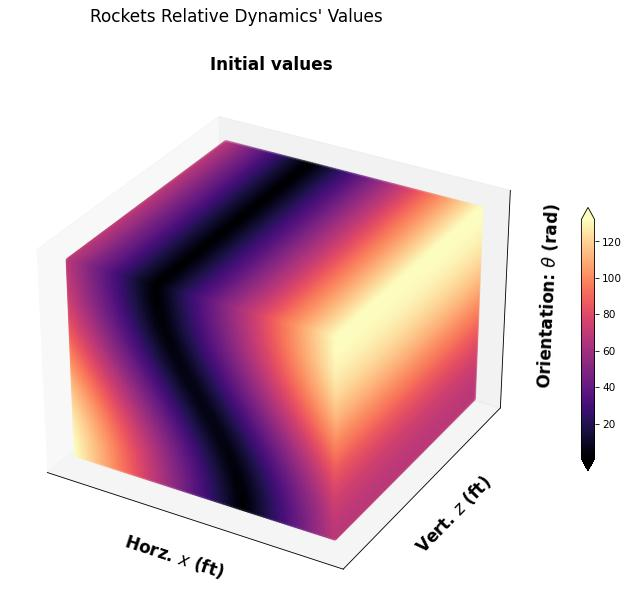
\includegraphics[width=0.48\textwidth]{figures/init_values.jpg} 
	\footnotesize{\caption{\textit{Left:} Motion of two rockets on a Cartesian $\bm{xz}$-plane with a thrust inclination in relative coordinates given by $\theta:=u_p- u_e$. \textit{Right:} Representation of the initial values as a heat map for the two rockets described in \eqref{eq:rocket_spatial_bounds}.}}
	\label{fig:rocket_relative}
\end{figure}
%
For a two-player differential game, let $\pursuer$ and $\evader$ share identical dynamics in a general sense so that we can freely choose the coordinates of $\pursuer$; however, $\evader$'s origin is a distance $\payoff$ away from $(x,z)$ at plane's origin (see Fig. \ref{fig:rocket_relative}) so that the $\pursuer\evader$ vector's inclination measured counterclockwise from the $\state$ axis is $\theta$. 

Hence, we may consider the current problem as a terminal pursuit-evasion \textit{differential} game, whereupon the game terminates when \textit{capture} occurs.  This eventual terminal represents the final \textit{overapproximated} (non)-capture surface for the $\pursuer-\evader$ game (to be shortly introduced). We desire that every \texttt{max} and \texttt{min} operations during a \textit{game of kind} are in the interior of the plane where motion exists; this way, no sudden changes from extremes are too aggravating in cost. 

Let the states of $\pursuer$ and $\evader$  be  $(\state_p, \state_e)$, respectively, driven by thrusts $(u_p, u_e)$ respectively  (see Figure \ref{fig:rocket_relative}). Fix the rockets' range so that what is left of the motion of either $\pursuer$ or $\evader$'s  is restricted to orientation on the $(x,{z})$ plane as illustrated in \autoref{fig:rocket_relative}. 
%
\noindent where $a$ and $g$ are respectively the acceleration and gravitational accelerations (in feet per square second) \footnote{We set $a=1 ft/sec^2$ and $g=32 ft/sec^2$ in our simulation.}.  
As long as $\evader$  remains within this target region or \textit{backward reachable tube} (or BRT), $\pursuer$ cannot cause damage or exercise an action of deleterious consequence on, say, the territory being guarded by $\evader$. Setting up $\evader$ to maximize a payoff quantity  with the largest possible margin or at least frustrate the efforts of $\pursuer$ with minimal collateral damage while the pursuer minimizes this quantity constitutes a terminal value \textit{optimal} differential game: there is no optimal pursuit without an optimal evasion. % since $\pursuer$ and $\evader$ are both executing motions as they see fit within the problem parameters. 

The motion of $\pursuer$  relative to $\evader$'s  along  the $(\state,\bm{z})$ plane includes the relative orientation, the control input, shown in \autoref{fig:rocket_relative} as $\theta=u_p- u_e$. Following the conventions in \autoref{fig:rocket_relative}, the game's relative equations of motion in \textit{reduced space}~\citet[\S 2.2]{Isaacs1965} was derived as (see~\citet[\S VI.A]{levpyconf})
is $\bm{x} = (x, {z}, {\theta})$ where ${\theta }\in \left[-\frac{\pi}{2}, \frac{\pi}{2}\right)$ and $(x,z) \in \bb{R}^2$ are 
%
%{subequations}
%\begin{align}
%\dot{\state} = 
%\begin{cases}
%\dot{x} &= a_p \cos \theta + u_e x, \\
%\dot{z} &=a_p \sin \theta + a_e + u_e x - g, \\%\\
%\dot{\theta} &= u_p -u_e.
%\end{cases}
%\label{eq:rocket_me}
%\end{align}
%\end{subequations}
%
\begin{align}
	\dot{\state} \implies \{ 
		\dot{x} = a_p \cos \theta + u_e x, \,\,
		\dot{z} =a_p \sin \theta + a_e + u_e x - g, \, \, %\\
		\dot{\theta} = u_p -u_e.
		\}
	\label{eq:rocket_me}
\end{align}

The capture radius of the origin-centered circle $\payoff$ (we set $\term=1.5$ ft) is $\|\pursuer \evader\|_2 $ so that $\term^2 =  x^2 + z^2.$
%
All capture points are specified by  the variational HJ PDE~\citet{Mitchell2005}:
%
\begin{align}
\dfrac{\partial \valuefunc}{\partial t} (\bm{x},t) + \min \left[0, \hamfunc\bigg(\state, \frac{\partial \term(\state, t)}{\partial \state}\bigg)\right] \le 0,
\label{eq:rockets_hji}
\end{align}
%
with Hamiltonian given by
%
\begin{align}
\hamfunc(\state, p) &= -\max_{u_e \in [\underline{u}_e, \bar{u}_e]} \min_{u_p \in [\underline{u}_p, \bar{u}_p].
} \begin{bmatrix}
p_1 & p_2 & p_3
\end{bmatrix} 
%
\begin{bmatrix}
a_p \cos \theta + u_e x \\
a_p \sin \theta + a_e + u_p x - g \\
u_p -u_e
\end{bmatrix}.
\label{eq:ham_def}
\end{align}
%
Here,  $p$ are the co-states, and $[\underline{u}_e, \bar{u}_e]$ denotes extremals that the evader must choose as input in response to the extremal controls that the pursuer plays \ie $[\underline{u}_p, \bar{u}_p]$. 
%
Rather than resort to analytical \textit{geometric reasoning}, we may analyze possibilities of behavior by either agent via a principled numerical simulation. This is the essence of this work. 
From \eqref{eq:ham_def}, set $\underline{u}_e = \underline{u}_p = \underline{u} \triangleq -1$ and $\bar{u}_p = \bar{u}_e = \bar{u} \triangleq +1$ so that $\hamfunc(\state, p)$ is
%
\begin{align}
& -\max_{u_e \in [\underline{u}_e, \bar{u}_e]} \min_{u_p \in [\underline{u}_p, \bar{u}_p]
} 
\begin{bmatrix}
p_1(a_p \cos \theta + u_e x) + \nonumber \\ p_2 (a_p \sin \theta + a_e + \nonumber \\ u_p x - g) + p_3 (u_p -u_e)
\end{bmatrix} \nonumber \\
%
%&= -a_p p_1 \cos \theta - a p_2 \sin \theta - a p_2 + g p_2 -\max_{u_e \in [\underline{u}_e, \bar{u}_e]} \min_{u_p \in [\underline{u}_p, \bar{u}_p]} \left(p_1 u_e + p_2 u_p x + p_3 (u_p - u_e)\right), \nonumber \\
%%
%&= -a_p p_1 \cos \theta - a p_2 \sin \theta - a p_2 + g p_2 -\bar{u} |p_1 x +  p_3 | + \underline{u} |p_2 x + p_3 |,  \nonumber \\
%
&\triangleq -a p_1 \cos \theta - p_2 (g - a - a\sin \theta) -\bar{u} |p_1 x +  p_3 |  + \underline{u} |p_2 x + p_3 |,
\label{eq:rocket_hamfunc}
\end{align}
%
where the last line follows from setting $a_e = a_p \triangleq a$. Thus, the rockets HJI equation~\eqref{eq:rockets_hji} becomes
%
\begin{align}
{\partial_t \valuefunc} (t; \bm{x}) + \min \left[0, (-a p_1 \cos \theta - p_2 (g - a - a\sin \theta) -  |p_1 x +  p_3 |  -|p_2 x + p_3 |)\right] \le 0,
\end{align}
%
where $p_1, p_2, p_3$ are the coefficients of the co-states obtained from \eqref{eq:hji_prox_pre}. A similar derivation can be obtained for the \eqref{eq:HJI-RCBRAT}. The initial values of the game is as illustrated in \autoref{fig:initial_values}.


\subsection{Numerical Integration Considerations}
We take the infinitesimal physics problem above and make it algorithmic first by discretizing the spatial and  temporal domains \ie 
%
\begin{align}
	(x, z) \in (-100, +100], \, {\theta} \in (-\pi/2, \pi/2], \,  t \in (0, 1],
	\label{eq:rocket_spatial_bounds}
\end{align}
 %
with $1000$  points along the temporal dimension and $\state_k - \state_{k-1}=1/100$ along the spatial dimensions, where $k \in \mathbb{N}$. All our codes are implemented in pytorch, that runs on an Azure Linux node with the cpu processor specification: Intel Xeon Silver 4208 at 2.1GHz and 65GB memory; The pytorch runs on a Ubuntu 22.04 operating system. 

We defined the target set as the top-left corner of the state space~\autoref{fig:initial_values}  and then run the Algorithm \ref{alg:rcbrt-sample} on a time range of $(0, 1]$ seconds; we chose Dirichlet boundary conditions
%
\begin{align}
	\bm{v}^\delta(0; \bm{x}) = \bm{g}(0; \bm{x}) \triangleq 0.
	\label{eq:rockets_dirichlet}
\end{align} 
%
The spatial gradients (co-states) were computed using the transformation \eqref{eq:prox_value_grad} which were then used in generating the Hamiltonian and subsequently the solution to the safe set using \eqref{eq:rockets_hji}. %In computing the values of the states in \eqref{eq:rocket_me} needed for computing the distance to the target region, we leverage the Runge-Kutta 45 ode integrator~\citet{}
 
% Care is taken not to combine the state components into one full spatial domain early on in the algorithm. We first sampled from each spatial component of \eqref{eq:rocket_spatial_bounds}, compute the values within the expectations in \eqref{eq:prox_value_grad}, and then compute the proximal for the full state space using the expectation-maximization algorithm~\citet{ExpectationMaximization}. The expectation-maximization algorithm proceeded as follows:
% %
% \begin{itemize}
% 	\item We first computed the logarithm of the observations
% \end{itemize} 
% 
% We do not employ a mesh or grid since the indices from which we sample are uniform across $x, z$ and $\theta$. The innards of the expression in \eqref{eq:prox_value_grad}  were first computed based on samples from the state space \eqref{eq:rocket_spatial_bounds}. %The expectation from the Gaussian distributions are computed with the expectation-maximization algorithm~\citet{JordanExpectimax}. %which yielded the proximal expression in terms of the spatial gradient of the value function.
\section{Conclude}
\label{sec:conclude}
We have presented a gradient-based nonconvex optimization scheme for computing the safe set of a two-person differential game. The gradient scheme is a zero order Moreau envelope optimization scheme whose extrema coincides with that of the HJ-Isaacs equation (which is non-convex in its Hamiltonian). We provided a means to optimize the Proximal operator of the Moreau envelope by adapting the ~\citet{HJMAD} algorithm and we note that once this extrema is found, determining the safe set amounts to searching within the resulting optimized terminal values of the HJI equation to see where the conditions of \eqref{eq:reachables} are fulfilled. We demonstrated a proof of concept with the relative motion of two rockets on a Cartesian grid where both players have control inputs: the evading player must avoid the pursuing player within a pre-specified time range while the pursuing player must try to capture the evader within the given time by maximizing time. In a best response strategy, each player responds to the control input of its adversarial player in a best-response strategy. Our results demonstrate the feasibility of our approach.



%%%%%%%%%%%%%%%%%%%%%%%%%%%%%%%%%%%%%%%%%%%%%%%%%%%%%%%%%%%%%%%%%%%%%%%%%%%%%%%%



\addtolength{\textheight}{-3cm}   % This command serves to balance the column lengths
                                  % on the last page of the document manually. It shortens
                                  % the textheight of the last page by a suitable amount.
                                  % This command does not take effect until the next page
                                  % so it should come on the page before the last. Make
                                  % sure that you do not shorten the textheight too much.

%%%%%%%%%%%%%%%%%%%%%%%%%%%%%%%%%%%%%%%%%%%%%%%%%%%%%%%%%%%%%%%%%%%%%%%%%%%%%%%%
\bibliographystyle{IEEEtran}
\bibliography{../TOMS/levtoms.bib}
\end{document}
